\documentclass[10pt]{beamer}

\usepackage{cmap}%allows cyrillic search in pdf
\usepackage[english,russian,ukrainian]{babel}
\usepackage[T2A]{fontenc}
\usepackage[utf8]{inputenc}

\usetheme[progressbar=frametitle]{metropolis}
\usepackage{appendixnumberbeamer}

\usepackage{booktabs}
%\usepackage[scale=2]{ccicons}

%\usepackage{pgfplots}
%\usepgfplotslibrary{dateplot}

%\usepackage{xspace}
%\newcommand{\themename}{\textbf{\textsc{metropolis}}\xspace}

\usepackage{wrapfig,graphicx,caption,subcaption,overpic,tikz}
\usepackage{amsmath, amssymb, amsfonts}
\usefonttheme[onlymath]{serif}
\usepackage{xcolor}

\title{ЕЛЕКТРОФІЗИЧНІ ВЛАСТИВОСТІ\\ БАГАТОФАЗНИХ ДИСПЕРСНИХ СИСТЕМ}
%\subtitle{A modern beamer theme}
% \date{\today}
\date{}
\author{Семенов Андрій Костянтинович}
\institute{Науковий керівник: к.ф.-м.н., доц. М. Я. Сушко\\
Кафедра теоретичної фізики та астрономії\\
Одеський національний університет імені І.І. Мечникова}
% \titlegraphic{\hfill\includegraphics[height=1.5cm]{logo.pdf}}

\begin{document}

\maketitle

%%%%%%%%%%%%%%%%%%%%%%%%%%%%%%%%%%%%%%%%%%%%%%%%%%%%%%
\begin{frame}{Мета роботи та поставлені задачі}

{\bf Мета роботи}:

{\footnotesize 
Побудова теорії ефективних електричних властивостей невпорядкованих дисперсних систем зі складною мікроструктурою (частинки та міжфазні шари).
% Побудова самоузгодженої макроскопічної теорії довгохвильового електричного відгуку немагнітних макроскопічно однорідних та ізотропних дисперсних систем.
}

{\bf Задачі}:

{\footnotesize 
% --- Узагальнити метод компактних груп (МКГ) на випадок провідних систем.

% --- Розробити послідовний метод електричної гомогенізації макроскопічно однорідних та ізотропних систем в рамках МКГ.

% --- Побудувати модель дисперсної системи сферичних частинок з морфологією типу тверде ядро--проникна оболонка.

% --- Протестувати адекватність розробленої теорії на числових даних.

% --- Проаналізувати характеристики перколяційної поведінки провідності та проникності в рамках теорії.

%--- Застосувати теоретичні результати до обробки експериментальних даних.

--- Розробити теорію електродинамічної гомогенізації невпорядкованих систем провідних частинок у рамках методу компактних груп (МКГ), для чого узагальнити та замкнути МКГ на випадок провідних частинок.

--- Проаналізувати в рамках цього підходу ефективні електричні властивості невпорядкованих систем частинок з морфологією тверде ядро--проникна оболонка та протестувати теорію шляхом порівняння з даними числових симуляцій.

--- Дослідити застосовність теорії до опису електричних властивостей твердих та полімерних композитних електролітів.

--- Дослідити застосовність теорії до опису електричної перколяції в дисперсноподібних композитах.

--- Виконати критичний аналіз диференціальної схеми обчислення ефективних електрофізичних параметрів гетерогенних систем.
}

\end{frame}

%%%%%%%%%%%%%%%%%%%%%%%%%%%%%%%%%%%%%%%%%%%%%%%%%%%%%%
\begin{frame}{Публікації}
\footnotesize
  \begin{itemize}
    \item
    Sushko M. Ya. Conductivity and permittivity of dispersed systems 
    with penetrable particle-host interphase~/ M.~Ya.~Sushko, 
    A.~K.~Semenov~// Cond. Matter. Phys. --- 2013. --- Vol.~16. --- No.~1. 
    --- P.~13401.
    
    \item
    Semenov~A.~K. On applicability of differential mixing rules for
      statistically homogeneous and isotropic dispersions~/ A.~K.~Semenov~//
      J. Phys. Commun. --- 2018. --- Vol.~2. --- No.~3. --- P.~035045.
    
    \item
    Sushko~M.~Ya. A mesoscopic model for the effective electrical 
    conductivity of composite polymeric electrolytes.~/ M.~Ya.~Sushko,
    A.~K.~Semenov~// J. Mol. Liq. --- 2019. --- Vol.~279. --- P.~677.
    
    \item
    Sushko~M.~Ya. Rigorously solvable model for the electrical conductivity of dispersions of hard-core--penetrable-shell particles and its applications~/
    M.~Ya.~Su\-shko, A.~K.~Semenov~//
    Phys. Rev. E --- 2019. --- Vol.~100. --- P.~052601.
  \end{itemize}

\end{frame}

%%%%%%%%%%%%%%%%%%%%%%%%%%%%%%%%%%%%%%%%%%%%%%%%%%%%%%
\begin{frame}{Участь у міжнародних конференціях та семінарах}
\vspace{-5pt}
{\footnotesize
\begin{enumerate}
\item 4-th International Conference on Statistical Physics: Modern Trends and Applications, Lviv (Ukraine), 2012.

\item 25-th International Conference: Disperse Systems, Odesa (Ukraine), 2012.

\item 5-th International Symposium: Methods and Applications of Computational Chemistry,  Kharkiv (Ukraine), 2013.

\item 6-th International Conference Physics  of  Liquid  Matter:  Modern Problems,  Kyiv (Ukraine), 2014.

\item 26-th International Conference: Disperse Systems,  Odesa (Ukraine), 2014.

\item 2015 International Young Scientists Forum on Applied Physics,  Dnipropetrovsk (Ukraine), 2015.

\item 27-th International Conference: Disperse Systems, Odesa (Ukraine), 2016.

\item International conference: Development of innovation in the technical, physical and mathematical fields of sciences, Mykolayiv (Ukraine), 2016.

\item 8-th International  Conference Physics  of  Liquid  Matter: Modern Problems, Kyiv (Ukraine), 2018.

\item 5-th International Conference on Statistical Physics: Modern Trends and Applications, Lviv (Ukraine), 2019.

\item 7-th International Conference: Nano\-technologies and Nanomaterials,  Lviv (Ukraine), 2019.

\item 28-th International Conference: Disperse Systems, Odesa (Ukraine), 2019.
\end{enumerate}
}

\end{frame}


%%%%%%%%%%%%%%%%%%%%%%%%%%%%%%%%%%%%%%%%%%%%%%%%%%%%%%
\begin{frame}{Актуальність роботи}

  \begin{itemize}
    \item Необхідність створення композитів із заданими характеристиками.
    \item Відсутність аналітичних послідовних багаточастинкових теорій дослідження електричних властивостей систем, що суттєво ускладнює їх розробку.
  \end{itemize}

\end{frame}

%%%%%%%%%%%%%%%%%%%%%%%%%%%%%%%%%%%%%%%%%%%%%%%%%%%%%%
% \begin{frame}{План доповіді}
%   \footnotesize
%   \setbeamertemplate{section in toc}[sections numbered]
%   \tableofcontents%[hideallsubsections]
%   \vspace{-25pt}
% \end{frame}


%%%%%%%%%%%%%%%%%%%%%%%%%%%%%%%%%%%%%%%%%%%%%%%%%%%%%
\section{Приклади досліджуваних систем}%%%%%%%%%%%%%%%%%%%%%Об'єкт та предмет дослідження?
%%%%%%%%%%%%%%%%%%%%%%%%%%%%%%%%%%%%%%%%%%%%%%%%%%%%%

\begin{frame}{Тверді композитні електроліти}
\footnotesize

%(Високопровідна оболонка, менш провідні ядро та матриця: $\sigma_2 \gg \sigma_1, \sigma_0$)
\vspace{5pt}

\begin{wrapfigure}{r}{0.4\textwidth}
\vspace{-25pt}
  \begin{center}
    \begin{overpic}[width=0.45\textwidth]{images/liang.eps}
         \put(60,15){$\rm LiI-Al_2O_3$}
    \end{overpic}
  \end{center}
\vspace{-50pt}
\end{wrapfigure}

---~Матриця: (полі)кристалічні галоїди металів (наприклад, літію, срібла, міді)\vspace{5pt}

--- Дисперсна фаза:  низькопровідні частинки (наприклад, оксид алюмінія).\vspace{5pt}

--- Провідність~чистих матриць $\sigma_0 \sim 10^{-10} \div 10^{-5}$ С/см. \vspace{5pt} 

--- Провідність~композитів на 1 - 3 порядки вище за $\sigma_0$. \vspace{5pt}

--- Зростання провідності копозиту зумовлене формуванням навколо диспергованих частинок областей з відносно високою провідністю $\sigma_2 (\gg \sigma_1, \sigma_0$) та зміною електричних властивостей матриці. \vspace{5pt}

--- Спадання – зменшенням об’ємної частки високопровідних областей при високих концентраціях непровідних частинок.

\end{frame}
%%%%%%%%%%%%%%%%%%%%%%%%%%%%%%%%%%%%%%%%%%%%%%%%%%%%%
\begin{frame}{Композитні полімерні електроліти}
\footnotesize

\begin{tikzpicture}
            \node[anchor=south west,inner sep=0] (image) at (0,0) {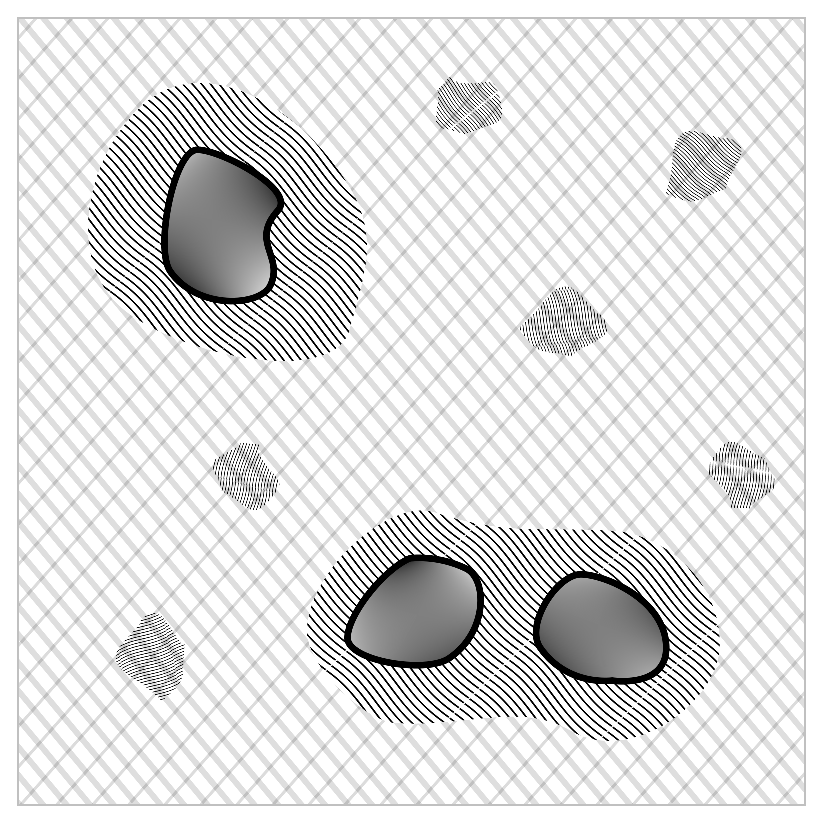
\includegraphics[width=0.45\textwidth]{images/PCE.eps}\qquad
            \includegraphics[width=0.45\textwidth]{images/PEO-OMPEO.eps}};
            \begin{scope}[x={(image.south east)},y={(image.north west)}]
                % \draw[red, very thick] (0.49,0.69) ellipse (0.08 and 0.05);
                % \draw[red, very thick] (0.6,0.72) ellipse (0.07 and 0.3);
                % \draw[red, very thick] (0.75,0.67) ellipse (0.12 and 0.06);
                \draw[->, thick] (0.18,0.1) -- (0.23,0.2);
                \draw[->, thick] (0.22,0.1) -- (0.33,0.2);
                \draw[->, thick] (0.16,0.1) -- (0.12,0.68);
                \node[] at (0.2,0.05) {Глобули PAAM};
                \draw[->, thick] (0.3,0.5) -- (0.18,0.62);
                \draw[->, thick] (0.31,0.37) -- (0.32,0.32);
                \node[] at (0.31,0.47) {Аморфізованй};
                \node[] at (0.25,0.41) {полімер};
                \draw[->, thick] (0.37,0.9) -- (0.41,0.83);
                \draw[->, thick] (0.35,0.9) -- (0.33,0.63);
                \node[] at (0.33,0.95) {Рештки PAAM};
            \end{scope}
\end{tikzpicture}

% \begin{wrapfigure}{r}{0.4\textwidth}
% \vspace{-25pt}
%   \begin{center}
%     \begin{overpic}[width=0.45\textwidth]{images/PEO-OMPEO.eps}
%          %\put(60,15){$\rm LiI/Al_2O_3$}
%     \end{overpic}
%   \end{center}
% \vspace{-30pt}
% \end{wrapfigure}

---~Дисперсійне середовище: полімери, що формують електродонорні зв’язки з різними неорганічними солями  (наприклад, $\rm LiClO_4$, $\rm NaI$, $\rm LiI$, $\rm CuCl$).

--- Дисперговані~частинки: провідні (наприклад, $\rm \beta-Al_2O_3$, $\rm RbAg_4I_5$, $\rm KAg_4I_5$) або непровідні (наприклад, $\rm \alpha-Al_2O_3$,  $\rm \gamma-Al_2O_3$, $\rm TiO_2$) неорганічні частики,
глобули полімеру іншого сорту.

% --- Провідність таких систем ($\sigma \sim 10^{-5} \div 10^{-3}$~С/см) на кілька порядків перевищує провідність чистих полімерних матриць ($\sigma_0 \sim 10^{-10} \div 10^{-5}$~С/см).\vspace{5pt}

--- Зростання провідності зумовлене формуванням навколо диспергованих частинок областей аморфізованого полімеру та зміною електричних властивостей матриці. 

\end{frame}

%%%%%%%%%%%%%%%%%%%%%%%%%%%%%%%%%%%%%%%%%%%%%%%%%%%%%
\begin{frame}{Системи, що демонструють перколяційний перехід}
\footnotesize

\vspace{-5pt}
\begin{wrapfigure}{r}{0.4\textwidth}
\vspace{-25pt}
  \begin{center}
    \begin{overpic}[width=0.42\textwidth]{images/grannan-sigma.eps}
         \put(60,70){$\rm KCl-Ag$}
    \end{overpic}
    \begin{overpic}[width=0.4\textwidth]{images/chen.eps}
         \put(20,80){$\rm KCl-Ag$}
    \end{overpic}
  \end{center}
\vspace{-25pt}
\end{wrapfigure}

---~Високопровідне~ядро (наприклад, $\rm Ag,\, Fe,\, Al$), менш провідна оболонка (наприклад, оксидні шари) та непровідна матриця  (наприклад, парафін, пресований порошок іонних кристалів): \vspace{-5pt}
$$\sigma_1 \geq \sigma_2 > \sigma_0.$$%\vspace{5pt}

--- %Провідність~чистих~матриць $\sigma_0 \sim 10^{-10} \div 10^{-2}$~С/см. 
Провідність композитів в залежності від компонентів може зростати на 3-8 порядків порівняно з провідністю чистої матриці. \vspace{5pt}

--- Різка зміна провідності пояснюється перекриттям оболонок та/або безпосереднім контактом провідних ядер частинок.\vspace{5pt}

--- Різка зміна проникності пояснюється утворенням розвинутої сітки конденсаторів в околі точки перколяційного переходу.

\end{frame}

%%%%%%%%%%%%%%%%%%%%%%%%%%%%%%%%%%%%%%%%%%%%%%%%%%%%%
\section{Ключові проблеми теоретичного аналізу та запропонована модель}
%%%%%%%%%%%%%%%%%%%%%%%%%%%%%%%%%%%%%%%%%%%%%%%%%%%%%
\begin{frame}{Ключові проблеми теоретичного аналізу}
--- Моделювання мікроструктури системи при наявності в ній різних фізико-хімічних механізмів, відповідальних за:
\begin{itemize}\footnotesize
    \item міжфазні ефекти: оксидні оболонки, утворення областей з високою концентрацією дефектів, подвійних електричних шарів тощо.
    \item матричні ефекти: зміна властивостей матриці внаслідок випадкового легування на етапі приготування зразків, аморфізація полімерної матриці диспергованими частинками та ін.
\end{itemize}

--- Розробка послідовної процедури електродинамічної гомогенізації, яка б:
  
\begin{itemize}\footnotesize
    \item була внутрішньо замкненою;
    \item ураховувала  багаточастинкові кореляційні та поляризаційні ефекти;
    \item обходила проблему невизначеності поняття індивідуальної поляризовності частинки зі складною морфологією.
\end{itemize}

\end{frame}


%%%%%%%%%%%%%%%%%%%%%%%%%%%%%%%%%%%%%%%%%%%%%%%%%%%%%
\begin{frame}{Модель структури: однорідні оболонки}

\begin{wrapfigure}{r}{0.35\textwidth}
\vspace{-25pt}
  \begin{center}
    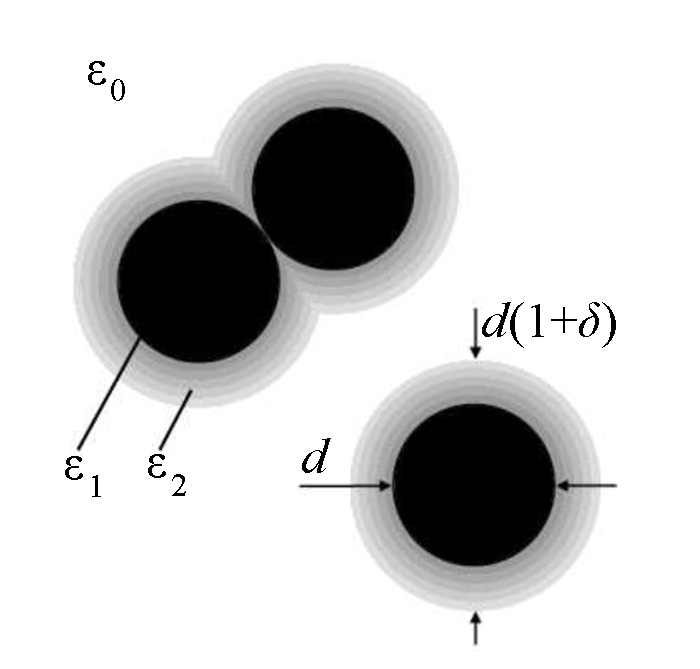
\includegraphics[width=0.35\textwidth]{images/particles-pen.eps}
    %\vspace{-10pt}
  \end{center}
\vspace{-25pt}
\end{wrapfigure}

% \begin{wrapfigure}{r}{0.45\textwidth}
% \vspace{-25pt}
%   \begin{center}
%     \includegraphics[width=0.45\textwidth]{images/Fig1_Microstructure_new5.eps}
%   \end{center}
% \vspace{-15pt}
% \end{wrapfigure}

\footnotesize
Розглядаємо \textbf{макроскопічно однорідні та ізотропні дисперсні системи частинок із морфологією тверде ядро--проникна оболонка:}
\vspace{-10pt}

% \begin{description}
%   \item[білі області] матриця 
%   \item[чорні області] тверді ядра
%   \item[сірі області] проникні оболонки 
% \end{description}
$$
    \hat{\varepsilon}({\bf r}) = \left\{ 
    \begin{array}{ll}
    \hat{\varepsilon}_1, l<R_1 & l = \min\limits_{1 \leq a \leq N} |{\bf r} - {\bf r}_a| \\
    \hat{\varepsilon}_2, R_1 < l < R_2 & R_1 = d/2 \\
    \hat{\varepsilon}_0, l > R_2 & R_2 = d(1+\delta)/2
    \end{array}    
    \right. 
$$

$$
    \hat{\varepsilon} ({\bf r}) = \hat{\varepsilon}_{\rm f} + \delta\hat{\varepsilon} ({\bf r})
$$

Для випадку $\hat{\varepsilon}_2 = const$:
\begin{equation*}
\begin{split}
    \delta\hat{\varepsilon}({\bf r}) = [1 - \Pi_2({\bf r})]\Delta\hat{\varepsilon}_0 + \Pi_1({\bf r}) \Delta\hat{\varepsilon}_1 
    + [\Pi_2({\bf r}) - \Pi_1({\bf r})]\Delta\hat{\varepsilon}_2,
\end{split}
\end{equation*}
де $\Delta\hat{\varepsilon}_q = \hat{\varepsilon}_{q} - \hat{\varepsilon}_{\rm f}\, (q=0,1,2),$ та введено такі характеристичні функції: \\
$\cdot\quad \Pi_1 ({\bf r}) = \sum\limits_{a=1}^N \chi_a^{(1)} ({\bf r})$ -- області, зайняті твердими ядрами ($\chi_a^{(1)}({\bf r})$ -- характеристична функція ядра $a$-ої частинки);\\
$\cdot\quad \Pi_2 ({\bf r}) = 1 - \prod\limits_{a=1}^N [1 - \chi_a^{(2)} ({\bf r})]$ -- області, зайнятої твердими ядрами разом з проникними оболонками ($\chi_a^{(2)}({\bf r})$ -- характеристична функція $a$-ої частинки (її ядра та оболонки)).
%\vspace{5pt}

%Для сферичних частинок $\chi_a^{(q)}({\bf r}) = \theta(R_q - |{\bf r} - {\bf r}_a|)$ -- ступінчаста функція Хевісайда.

\end{frame}

%%%%%%%%%%%%%%%%%%%%%%%%%%%%%%%%%%%%%%%%%%%%%%%%%%%%%
\begin{frame}{Модель структури: неоднорідні оболонки}

%Для випадку $\hat{\varepsilon}_2 = \hat{\varepsilon}_2({\bf r})$:

\footnotesize
Припускаємо, що використання електрично неоднорідних проникних оболонок, що підкоряються певному правилу домінування, дозволяє ефективно врахувати як міжфазні, так і матричні ефекти.

\begin{wrapfigure}{r}{0.35\textwidth}
\vspace{-20pt}
  \begin{center}
    \includegraphics[width=0.35\textwidth]{images/2shell.png}
  \end{center}
\vspace{-25pt}
\end{wrapfigure}
\begin{equation*}\label{eq:distr1}
\hat{\varepsilon}({\bf r})=\begin{cases}
\hat{\varepsilon}_1, & l<R_1, \qquad l=\min\limits_{1 \leq a \leq N} |{\bf r} - {\bf r}_a| \\
\hat{\varepsilon}_{2,1}, &  R_1<l<R_{2,1},\\
{\hat{\varepsilon}_{2,m}}, & { R_{2,m-1}<l<R_{2,m}, \,2 \leq m \leq M},\\
\hat{\varepsilon}_0, & l>R_{2,M}.
\end{cases}
\end{equation*}
Відповідно
\begin{equation*}
\begin{split}
\delta\hat{\varepsilon} ({\bf r}) = \left[1- \Pi_{2,M}({\bf
r})\right] \Delta\hat{\varepsilon}_0
+ \Pi_1({\bf r}) \Delta\hat{\varepsilon}_1
+  \left[\Pi_{2,1}({\bf r})
-\Pi_1({\bf r})  \right] \Delta\hat{\varepsilon}_{2,1} \\
+ {\sum\limits_{m=2}^M  \left[ \Pi_{2,m}({\bf r}) -
\Pi_{2,m-1}({\bf r}) \right] \Delta\hat{\varepsilon}_{2,m}},
\end{split}
\end{equation*}
де $\Pi_{2,m} ({\bf r}) = 1 - \prod\limits_{a=1}^N [1 - \chi_a^{(2,m)} ({\bf r})]$ -- характеристична функція області, зайнятої твердими ядрами разом з $m$-ими проникними оболонками ($\chi_a^{(2,m)}({\bf r})$ -- характеристична функція $a$-ого ядра та його $m$-ої оболонки).

% Для сферичних частинок $\phi$ знайдено статистичними методами в рамках суперпозиційного підходу Кірквуда, строгого на рівні третього вірального коефіцієнта  [P.~Rikvold, G.~Stell, J. Coll. and Int. Sci. {\bf 108} (1985) 158]
% \begin{equation}\label{effectiveconcentration}
% \begin{split}
% \phi(c,\delta)= 1-
% (1 - c)\,\exp\left[{-\frac{((1+\delta)^3 -
% 1)c}{1-c}}\right] \\
%  \times  \exp\left\{
% - \frac{3(1 + \delta)^3
% c^2}{2(1 - c)^3} \left[2 - \frac{3}{1+\delta} +
% \frac{1}{(1+\delta)^3} \right. \right. \\
% - \left. \left. \left( \frac{3}{1+\delta} -
% \frac{6}{(1+\delta)^2} + \frac{3}{(1+\delta)^3}\right) c
% \right]\right\}. 
% \end{split}
% \end{equation}


\end{frame}

%%%%%%%%%%%%%%%%%%%%%%%%%%%%%%%%%%%%%%%%%%%%%%%%%%%%%%%%%%%%%%%%%%%%%%%%%%%%%%%%%%%%%%%%%%%
\section{Теоретична реалізація моделі}%%%%%%%%%%%%%%%%%%%%%%
%%%%%%%%%%%%%%%%%%%%%%%%%%%%%%%%%%%%%%%%%%%%%%%%%%%%%%%%%%%%%%%%%%%%%%%%%%%%%%%%%%%%%%%%%%%
\begin{frame}{Основні припущення та співвідношення}

\begin{list}{$\bullet$}{\leftmargin=1em \itemindent=0em}\footnotesize

\item
Частота тестуючого поля $\omega$ достатньо мала, щоб можна було знехтувати діелектричними втратами: 
$$
    \hat{\varepsilon} = \varepsilon + i \frac{4\pi\sigma}{\omega},
$$
де $\varepsilon$ -- дійсна частина діелектричної проникності; $\sigma$ -- статична провідність

\item 
Ефективну квазістатичну $\hat{\varepsilon}_{\rm eff}$ визначаємо із співвідношення
\begin{equation}\label{eq:effcomplex} 
\langle {\bf{J}} ({\bf{r}})\rangle =
-i\frac{\omega}{4\pi}\langle \hat{\varepsilon} ({\bf{r}}) {\bf{E}}
({\bf{r}}) \rangle = -i\frac{\omega}{4\pi} \hat{\varepsilon}_{\rm
eff} \langle {\bf{E}} ({\bf{r}}) \rangle,
\end{equation}
де ${\bf J}({\bf{r}})$ та ${\bf E}({\bf{r}})$ -- локальні значення щільності комплексного струму та напруженості електричного поля; кутові дужки позначають статистичне усереднення за положеннями частинок.

% \item 
% Розрахунки ${\bf J}({\bf{r}})$ та ${\bf E}({\bf{r}})$ виконуються в рамках {\bf методу ``компактних груп неоднорідностей''}.

\end{list}

\end{frame}
%%%%%%%%%%%%%%%%%%%%%%%%%%%%%%%%%%%%%%%%%%%%%%%%%%%%%
\begin{frame}{Знаходження ${\bf E} ({\bf r})$}
\footnotesize
%[М.Я. Сушко, ЖЭТФ {\bf 132} (2007) 478; J. %Phys. D: Appl. Phys. {\bf 42} (2009) 155410; %Phys. Rev. E {\bf 96} (2017) 062121]

\begin{list}{$\bullet$}{\leftmargin=1em \itemindent=0em}
\item
Напруженість електричного поля ${\bf E} ({\bf r})$ електромагнітної хвилі в $\cal{S}$ описується інтегральним рівнянням
\begin{equation}\label{eq:propogating_field_integral} 
{\rm {\bf E}}({\rm {\bf r}}) = {\rm {\bf E}}_{0} ({\rm
{\bf r}}) - {\int\limits_{V} {d{\rm {\bf {r}'}}\,}} {\rm T}(|{\rm {\bf
r}}-{\rm {\bf {r}'}}|) k_{0}^{2} \delta \hat{\varepsilon} ({\rm
{\bf {r}'}})\,{\rm {\bf E}}({\rm {\bf {r}'}}),
\end{equation}
де $k_0=\omega/c$ -- модуль хвильового вектора ${\bf k}_0$ у вакуумі; ${\bf E}_0 ({\bf r}) = {\bf E}_0 \exp{(i\, {\bf k} \cdot{\bf r})}$ та ${\bf k} = \hat{\varepsilon}_{\rm f}^{1/2} {\bf k}_0$ (з ${\rm Im}{\hat{\varepsilon}_{\rm f}}^{1/2} \geq 0$) -- поле та хвильовий вектор падаючої хвилі в $\cal{M}$;
${\rm T}(r)$ -- пропагатор електричного поля (тензор Гріна). 

\item
При обчисленні інтеграла (\ref{eq:propogating_field_integral}) підінтегральний пропагатор ${\rm T}(r)$ заміняємо його розкладом [W. Weiglhofer, Am. J. Phys. {\bf 57} (1989) 455] на сингулярну та головну частини:
\begin{eqnarray}\label{eq:propog_representation} 
{\widetilde T}_{\alpha\beta} ({\rm {\bf
r}}) = \frac{1}{3k^{2}} \delta_{\alpha\beta} \delta ({\rm {\bf
r}})\,e^{ikr} + \frac{1}{4\pi k^{2}}
\left(\frac{1}{r^3}-\frac{ik}{r^2}\right)\nonumber\\
\times\left( \delta _{\alpha\beta} - 3e_{\alpha} e_{\beta}
\right)\,e^{ikr} - \frac{1}{4\pi r}\left( {\delta _{\alpha\beta} -
e_{\alpha} e_{\beta}} \right)\,e^{ikr},
\end{eqnarray}
де $\delta({\bf r})$ -- дельта-фукція Дірака; $\delta_{\alpha\beta}$ -- символ Кронекера; $e_\alpha = r_\alpha/|{\bf r}|$.

\end{list}

\end{frame}
%%%%%%%%%%%%%%%%%%%%%%%%%%%%%%%%%%%%%%%%%%%%%%%%%%%%%
\begin{frame}{Фізична інтерпритація методу компактних груп}

\scriptsize{
[М.Я. Сушко, ЖЭТФ {\bf 132} (2007) 478; J. Phys. D: Appl. Phys. {\bf 42} (2009) 155410; Phys. Rev. E {\bf 96} (2017) 062121]
}
\vspace{-5pt}
\begin{figure}
          \begin{center}
            \begin{overpic}[width=0.75\textwidth]{images/CGA.eps}
                 \put(2,40){$\cal{D}$}
                 \put(57,40){$\cal{M}$}
                 \put(70,35){$\cal{D}$}
                 \put(48.5,25){$\cal{S}$}
                 \put(75,0.7){$L \ll \lambda$}
            \end{overpic}
          \end{center}
\end{figure}

\begin{list}{$\bullet$}{\leftmargin=1em \itemindent=0em}\footnotesize

\item 
Припускаємо, що електричний відгук реальної дисперсної системи $\cal{D}$ еквівалентний відгуку допоміжної системи $\cal{S}$, утвореної диспергуванням компонентів $\cal{D}$ в деяку однорідну матрицю $\cal{M}$, з проникністю $\hat{\varepsilon}_{\rm f}$.

\item

$\cal{S}$ розглядаємо як сукупуність макроскопічних областей (компактних груп), лінійні розміри $L$ яких набагато менші ніж довжина хвилі $\lambda$ в $\cal{M}$, але досить великі, щоб формувати властивості всієї $\cal{S}$.

% \item
% Розподіл комплексної діелектричної проникності в $\cal{S}$ моделюємо у вигляді
% $$
%     \hat{\varepsilon} ({\bf r}) = \hat{\varepsilon}_{\rm f} + \delta\hat{\varepsilon} ({\bf r}),
% $$
% де $\hat{\varepsilon}_{\rm f}$ -- проникність $\cal{M}$; $\delta\hat{\varepsilon} ({\bf r})$ -- кусково-неперервна функція, що враховує внесок компактної групи частинок, розташованої в точці $\bf r$.

\end{list}

\end{frame}

%%%%%%%%%%%%%%%%%%%%%%%%%%%%%%%%%%%%%%%%%%%
\begin{frame}{Основний результат для $\langle {\bf J} \rangle$, $\langle {\bf E} \rangle$ та  $\hat{\varepsilon}_{\rm eff}$}
\footnotesize

\begin{list}{$\bullet$}{\leftmargin=1em \itemindent=0em}

\item
Після переходу до квазістатичного наближення із урахуванням симетрії парних кореляційних функцій для розглядуваних систем отримуємо:
\begin{equation}\label{eq:Eaveraged}
\langle \mathbf{E} (\mathbf{r}) \rangle = \left\langle \frac{ 3
\hat{\varepsilon}_{\rm f}  }{3 \hat{\varepsilon}_{\rm f}
+ \delta\hat{\varepsilon}({\bf r})} \right\rangle \mathbf{E}_0 ,
\end{equation}
\begin{equation}\label{eq:Caveraged}
\langle \mathbf{J}  (\mathbf{r}) \rangle = -i \frac{\omega}{4\pi}
\, \hat{\varepsilon}_{\rm f}\left[1+ 2\left\langle \frac{
\delta\hat{\varepsilon}({\bf r}) }{3 \hat{\varepsilon}_{\rm f}
+ \delta\hat{\varepsilon}({\bf r})} \right\rangle \right] \mathbf{E}_0.
\end{equation}

\item
З граничних умов для нормальних компонент електричного поля на поверхні розділу $\cal{M}$ та $\cal{D}$:
\begin{equation} \label{eq:boundarycondition}
\hat{\varepsilon}_{\rm
f} {\mathbf{E}}_{0n} = \hat{\varepsilon}_{\rm eff}
\left\langle{\mathbf{E}}({\mathbf{r}})\right\rangle_n.
\end{equation}
За умови, що $\hat{\varepsilon}_{\rm f} \neq 0$, дістаємо:
\begin{equation} \label{eq:ef} 
\hat{ \varepsilon}_{\rm f} = \hat{ \varepsilon}_{\rm eff},
\end{equation}
що дає рівняння для знаходження $\hat{\varepsilon}_{\rm eff}$:
\begin{equation} \label{eq:equation}
\boxed{
\left\langle \frac{\delta\hat{\varepsilon}({\bf r}) }{3 \hat{\varepsilon}_{\rm eff} + \delta\hat{\varepsilon}({\bf r})} \right\rangle = 0.
}
\end{equation}


\end{list}

\end{frame}

%%%%%%%%%%%%%%%%%%%%%%%%%%%%%%%%%%%%%%%%%%%%%%%%%%%%%
\begin{frame}{Основні теоретичні результати для обраної моделі $\delta\hat{\varepsilon}$}
\footnotesize

\begin{list}{$\bullet$}{\leftmargin=1em \itemindent=0em}
\item
Рівняння для $\hat{\varepsilon}_{\rm eff}$ у випадку \textbf{однорідних оболонок}:
\begin{equation}\label{eq:uniformshell}
\boxed{
\left[1-\phi(c, \delta)\right]\frac{\hat{\varepsilon}_0
-\hat{\varepsilon}_{\rm eff}}{2\hat{\varepsilon}_{\rm
eff}+\hat{\varepsilon}_0} + c\,\frac{\hat{\varepsilon}_1
-\hat{\varepsilon}_{\rm eff}}{2\hat{\varepsilon}_{\rm
eff}+\hat{\varepsilon}_1}
+\left[\phi(c, \delta)-c\right]\frac{\hat{\varepsilon}_2
-\hat{\varepsilon}_{\rm eff}}{2\hat{\varepsilon}_{\rm
eff}+\hat{\varepsilon}_2}=0, 
}
\end{equation}
де $c = \langle \Pi_1 \rangle$ -- об'ємна концентрація ядер; $\phi = \langle \Pi_2 \rangle$ -- об'ємна концентрація ядер з оболонками. 

\item
Для \textbf{неоднорідних оболонок} після переходу до границі $M \to \infty$ ($\delta_M = const$):
\begin{equation}\label{eq:nonuniformshell}
\boxed{
\left[1-\phi(c, \delta_M)\right]\frac{\hat{\varepsilon}_0
-\hat{\varepsilon}_{\rm eff}}{2\hat{\varepsilon} _{\rm
eff}+\hat{\varepsilon}_0}+ c\,\frac{\hat{\varepsilon}_1
-\hat{\varepsilon}_{\rm eff}}{2\hat{\varepsilon}_{\rm
eff}+\hat{\varepsilon}_1}
+\int\limits_0^{\delta_M}\frac{\partial \phi(c,u)}{\partial
u}\frac{\hat{\varepsilon}_2 (u) -\hat{\varepsilon}_{\rm
eff}}{2\hat{\varepsilon}_{\rm eff}+\hat{\varepsilon}_2 (u)}\,du
=0
}
\end{equation}

\item
За умови, що  $|\sigma_{\rm eff}-\sigma_{ q}|  \gg  
\left(2\varepsilon_{\rm eff} +\varepsilon_q \right) \omega/4\pi$ для всіх $q=0,1,2$,  рівняння для квазістатичної провідності мають вигляд:
\begin{equation*}\label{eq:conductivity}
\boxed{
\left[1-\phi(c, \delta)\right]\frac{\sigma_0 -\sigma_{\rm
eff}}{2\sigma_{\rm eff}+\sigma_0} + c\,\frac{\sigma_1 -\sigma_{\rm
eff}}{2\sigma_{\rm eff}+\sigma_1} 
+\left[\phi(c, \delta)-c\right]\frac{\sigma_2 -\sigma_{\rm
eff}}{2\sigma_{\rm eff}+\sigma_2}=0. 
}
\end{equation*}
\begin{equation*}\label{eq:nonuniformconductivity}
\boxed{
\left[1-\phi(c, \delta_M)\right]\frac{\sigma_0 -\sigma_{\rm
eff}}{2\sigma _{\rm eff}+\sigma_0}+ c\,\frac{\sigma_1 -\sigma_{\rm
eff}}{2\sigma_{\rm eff}+\sigma_1} 
+\int\limits_0^{\delta_M}\frac{\partial \phi(c,u)}{\partial
u}\frac{\sigma_2 (u) -\sigma_{\rm eff}}{2\sigma_{\rm eff}+\sigma_2
(u)}\,du =0.
}
\end{equation*}
У статичному випадку цей результат є \textbf{строгим}.

\end{list}

\end{frame}


%%%%%%%%%%%%%%%%%%%%%%%%%%%%%%%%%%%%%%%%%%%%%%%%%%%%%%%%%%%%%%%%%%%%%%%%%%%%%%%%%%%%%%%%%%%
\section{Тестування моделі на результатах числових симуляцій}%%%%%%%%%%%%%%%%%%%%%%%%%%%%%%%
%%%%%%%%%%%%%%%%%%%%%%%%%%%%%%%%%%%%%%%%%%%%%%%%%%%%%%%%%%%%%%%%%%%%%%%%%%%%%%%%%%%%%%%%%%

\begin{frame}{Тестування теорії на результатах симуляцій RRN}

{\footnotesize
Симуляції: [M. Siekierski et al., Electrochimica Acta {\bf 50} (2005) 3796; 
J. New Mat. Electrochem. Systems {\bf 9} (2006) 375;
J. Pow. Sour. {\bf 173} (2007) 748]
}

\begin{figure}[tb]
    \centering
    \includegraphics[width=0.7\textwidth]{images/RRN.png}
    \caption{Схематичне зображення алгоритму Random Resistor Network (RRN): a) модельна система типу ядро-оболонка; b) її апроксимація системою кубів; c) отримана тривимірна кубічна гратка резисторів.\\ {\footnotesize (Рис. взято з [M. Siekierski, K. Nadara, J. Pow. Sour. {\bf 173} (2007) 748])}}
\end{figure}
\vspace{-10pt}
Концентрації ядер в системах a) та b) рівні: $c=c'$, тоді відповідні відносні товщини будуть зв'язані співвідношенням:
$$
    \delta = K\delta'
$$
$$
    k \leq K \leq 1, \qquad k=(\pi/6)^{1/3}
$$

\end{frame}

%%%%%%%%%%%%%%%%%%%%%%%%%%%%%%%%%%%%%%%%%%%%%%%%%%%%%
%{\setbeamertemplate{frame footer}{Симуляції: [M. Siekierski, K. Nadara, J. Pow. Sour. {\bf 173} (2007) 748]}
\begin{frame}{Тестування зв'язку геометричних параметрів моделей a) та b)}

{ Об'ємні концентрації оболонок товщиною $t=5$~мкм як функції $c$.}
\vspace{-5pt}

\scriptsize{Симуляції: [M. Siekierski, K. Nadara, J. Pow. Sour. {\bf 173} (2007) 748]}
\vspace{-5pt}

\footnotesize
\begin{columns}[T,onlytextwidth]
    \column{0.5\textwidth}
      \begin{figure}
        \centering
        \qquad Діаметр ядра $d=7$~мкм
        \includegraphics[width=0.99\textwidth]{images/Fig2_SiekierskiShell_107.eps}
      \end{figure}

    \column{0.5\textwidth}
      \begin{figure}
        \centering
        \qquad Діаметри ядер $d=3,5,9$~мкм
        \includegraphics[width=0.99\textwidth]{images/Fig3_SiekierskiShell_103-9.eps}
      \end{figure}
\end{columns}

\begin{columns}[T,onlytextwidth]
    \column{0.45\textwidth}
      \vspace{5pt}
    %   Середньоквадратична похибка:
    %   $$
    %     \Delta_a = \sqrt{\frac{1}{N}\sum\limits_{i=1}^N (a_i - \tilde{a}_i)^2}
    %   $$
    Для сферичних частинок $\phi$ знайдено статистичними методами в рамках суперпозиційного підходу Кірквуда, строгого на рівні третього вірального коефіцієнта  [P.~Rikvold, G.~Stell, J. Coll. and Int. Sci. {\bf 108} (1985) 158]

    \column{0.55\textwidth}
    %   \begin{table}
    %     %\caption{Largest cities in the world (source: Wikipedia)}
    %     \begin{tabular}{ll}
    %       \toprule
    %       Експеримент & MSE\\
    %       \midrule
    %       $\circ$ $t=0$~мкм & 0.0024\\
    %       $\blacklozenge$ $d=3$~мкм & 0.0053\\
    %       $\blacksquare$ $d=5$~мкм & 0.011\\
    %       $\blacktriangle$ $d=7$~мкм & 0.014\\
    %       $\bullet$ $d=9$~мкм & 0.0097\\
    %       \bottomrule
    %     \end{tabular}
    %   \end{table}
    \begin{equation*}\label{effectiveconcentration}
    \begin{split}
    \phi(c,\delta)= 1-
    (1 - c)\,\exp\left[{-\frac{((1+\delta)^3 -
    1)c}{1-c}}\right] \\
     \times  \exp\left\{
    - \frac{3(1 + \delta)^3
    c^2}{2(1 - c)^3} \left[2 - \frac{3}{1+\delta} +
    \frac{1}{(1+\delta)^3} \right. \right. \\
    - \left. \left. \left( \frac{3}{1+\delta} -
    \frac{6}{(1+\delta)^2} + \frac{3}{(1+\delta)^3}\right) c
    \right]\right\}. 
    \end{split}
    \end{equation*}
\end{columns}

\end{frame}
%}
%%%%%%%%%%%%%%%%%%%%%%%%%%%%%%%%%%%%%%%%%%%%%%%%%%%%%
%{\setbeamertemplate{frame footer}{Симуляції: [M. Siekierski, K. Nadara, Electrochimica Acta {\bf 50} (2005) 3796]}
\begin{frame}{Порівняння з числовими даними з провідності}
Концентраційна залежність ефективної провідності при фіксованих $t$ (зліва) та $d$ (справа) з різними значеннями $K$.
\vspace{-5pt}

\scriptsize{Симуляції: [M. Siekierski, K. Nadara, Electrochimica Acta {\bf 50} (2005) 3796]}

\footnotesize
\begin{columns}[T,onlytextwidth]
    \column{0.5\textwidth}
      \begin{figure}
        \centering
        { \qquad Товщина оболонки $t=5$~мкм}
        \includegraphics[width=0.99\textwidth]{images/Fig6_Siekierski_HomogeneousLayers_t_fixed.eps}
      \end{figure}

    \column{0.5\textwidth}
      \begin{figure}
        \centering
        { \qquad Діаметр ядра $d=5$~мкм}
        \includegraphics[width=0.99\textwidth]{images/Fig7_Siekierski_HomogeneousLayers_d_fixed.eps}
      \end{figure}
\end{columns}

\begin{columns}[T,onlytextwidth]
    \column{0.6\textwidth}
      \vspace{10pt}
      Середньоквадратична відносна похибка:
      $$
        \bar{\Delta}_a = \sqrt{\frac{1}{N}\sum\limits_{i=1}^N \left( \frac{a_i - \tilde{a}_i}{a_i} \right)^2}
      $$

    \column{0.4\textwidth}
      \begin{table}
        %\caption{Largest cities in the world (source: Wikipedia)}
        \begin{tabular}{ll}
          \toprule
          Експеримент & $\max \bar{\Delta}_{\sigma_{\rm eff}/\sigma_0}$\\
          \midrule
          $t=5$~мкм & 0.40 | 0.048\\
          $d=5$~мкм & 0.35 | 0.019\\
          \bottomrule
        \end{tabular}
      \end{table}
\end{columns}
\end{frame}
%}

%%%%%%%%%%%%%%%%%%%%%%%%%%%%%%%%%%%%%%%%%%%%%%%%%%%%%
%{\setbeamertemplate{frame footer}{Симуляції: [M. Siekierski et al., J. New Mat. Electrochem. Systems {\bf 9} (2006) 375]}
\begin{frame}{Тестування моделі для випадку неоднорідних оболонок}
Концентраційна залежність ефективної провідності з різними значеннями $K$ для гаусового профілю оболонок.
\vspace{-5pt}

\scriptsize{Симуляції: [M. Siekierski et al., J. New Mat. Electrochem. Systems {\bf 9} (2006) 375]}

\footnotesize
\begin{columns}[T,onlytextwidth]
    \column{0.5\textwidth}
      \begin{figure}
        \centering
        { \qquad Товщина оболонки $t=5$~мкм}
        \includegraphics[width=0.99\textwidth]{images/Fig10_Siekierski_t_fixed.eps}
        $\max \bar{\Delta}_{\sigma_{\rm eff}/\sigma_0} \approx 0.41\,|\,0.048$\\
      \end{figure}

    \column{0.5\textwidth}
      \begin{figure}
        \centering
        { \qquad Діаметр ядра $d=5$~мкм}
        \includegraphics[width=0.99\textwidth]{images/Fig11_Siekierski_d_fixed.eps}
        $\max \bar{\Delta}_{\sigma_{\rm eff}/\sigma_0} \approx 0.28\,|\,0.28$
      \end{figure}
\end{columns}

\end{frame}
%}

%%%%%%%%%%%%%%%%%%%%%%%%%%%%%%%%%%%%%%%%%%%%%%%%%%%%%%%%%%%%%%%%%%%%%%%%%%%%%%%%%%%%%%%%%%%
\section{Застосування моделі до аналізу ефективної провідності композитних електролітів}%%%%%%%%%%%%%%%%%%%%%%%%%%%%%%%
%%%%%%%%%%%%%%%%%%%%%%%%%%%%%%%%%%%%%%%%%%%%%%%%%%%%%%%%%%%%%%%%%%%%%%%%%%%%%%%%%%%%%%%%%%
%\subsection{Тестування моделі на числових результатах симуляцій}

%%%%%%%%%%%%%%%%%%%%%%%%%%%%%%%%%%%%%%%%%%%%%%%%%%%%%
%\subsection{Порівняння з експериментальними даними}

%{\setbeamertemplate{frame footer}{Експеримент: [C.C. Liang, J. Electrochem. Soc., {\bf 120} (1973) 1289]}
\begin{frame}{Порівняння теорії з експериментальними даними -- 1}
Концентраційна залежність провідності систем $\rm LiI-Al_2O_3$.
\vspace{-5pt}

\scriptsize{Експеримент: [C.C. Liang, J. Electrochem. Soc., {\bf 120} (1973) 1289]}
\vspace{-10pt}

\footnotesize
\begin{columns}[T,onlytextwidth]
    \column{0.5\textwidth}
      \begin{figure}
        \centering
        %{ \qquad Діаметр ядра $d=7$~мкм}
        %\includegraphics[width=0.99\textwidth]{images/Fig12_Liang_LiI-Al2O3-Processing.eps}
        \begin{overpic}[width=0.95\textwidth]{images/Fig12_Liang_LiI-Al2O3-Processing.eps}
                 \put(45,87){\scriptsize $\sigma_0 \approx 2.5 \times 10^{-7}$~С/см}
        \end{overpic}
      \end{figure}
      \vspace{-10pt}
      % подвійні оболонки - $\bar{\Delta}_{\sigma_{\rm eff}/\sigma_0} \approx 0.143$\\
      % неперервний профіль - $\bar{\Delta}_{\sigma_{\rm eff}/\sigma_0} \approx 0.163$
      Точкова лінія -- електрично однорідна оболонка.\\
      Штрихована лінія -- подвійна (ступінчата) оболонка.\\
      Неперервна лінія -- гладкий профіль провідності.
      

    \column{0.5\textwidth}
    \vspace{5pt}
        \begin{tikzpicture}
            \node[anchor=south west,inner sep=0] (image) at (0,0) {\includegraphics[width=0.95\textwidth]{images/Fig13_Liang_LiI-Al2O3-Profile.eps}};
            \begin{scope}[x={(image.south east)},y={(image.north west)}]
                \node[] at (0.55,1.05) {Одночастинковий профіль провідності};
            \end{scope}
        \end{tikzpicture}
        Концентраційна залежність провідності матриці $\sigma_0^*$:
        \vspace{-5pt}
        \begin{eqnarray*}
        &&(1 - \phi(c,\delta_1))\frac{\sigma_0^* - \sigma_{\rm
        eff}}{2\sigma_{\rm eff} + \sigma_0^*}=\nonumber\\
        &&(1 - \phi(c,\delta_2))
        \frac{\sigma_0 - \sigma_{\rm eff}}{2\sigma_{\rm eff} + \sigma_0}
         \nonumber\\
        &&+ (\phi(c,\delta_2) - \phi(c,\delta_1)) \frac{\sigma_{2,2} -
        \sigma_{\rm eff}}{2\sigma_{\rm eff} + \sigma_{2,2}}
        \end{eqnarray*}
      
\end{columns}

\end{frame}
%}
\begin{frame}{Порівняння теорії з експериментальними даними -- 1}
Концентраційна залежність провідності систем $\rm LiI-Al_2O_3$.
\vspace{-5pt}

\scriptsize{Експеримент: [C.C. Liang, J. Electrochem. Soc., {\bf 120} (1973) 1289]}
\vspace{-10pt}

\footnotesize
\begin{columns}[T,onlytextwidth]
    \column{0.5\textwidth}
      \begin{figure}
        \centering
        %{ \qquad Діаметр ядра $d=7$~мкм}
        %\includegraphics[width=0.99\textwidth]{images/Fig12_Liang_LiI-Al2O3-Processing.eps}
        \begin{overpic}[width=0.95\textwidth]{images/Fig12_Liang_LiI-Al2O3-Processing.eps}
                 \put(45,87){\scriptsize $\sigma_0 \approx 2.5 \times 10^{-7}$~С/см}
        \end{overpic}
      \end{figure}
      \vspace{-10pt}
      % подвійні оболонки - $\bar{\Delta}_{\sigma_{\rm eff}/\sigma_0} \approx 0.143$\\
      % неперервний профіль - $\bar{\Delta}_{\sigma_{\rm eff}/\sigma_0} \approx 0.163$
      Точкова лінія -- електрично однорідна оболонка.\\
      Штрихована лінія -- подвійна (ступінчата) оболонка.\\
      Неперервна лінія -- гладкий профіль провідності.
      

    \column{0.5\textwidth}
    \vspace{5pt}
        \begin{tikzpicture}
            \node[anchor=south west,inner sep=0] (image) at (0,0) {\includegraphics[width=0.95\textwidth]{images/Fig13_Liang_LiI-Al2O3-Profile.eps}};
            \begin{scope}[x={(image.south east)},y={(image.north west)}]
                %\draw[red,ultra thick,rounded corners] (0.62,0.65) rectangle (0.78,0.75);
                \node[] at (0.55,1.05) {Одночастинковий профіль провідності};
                \draw[red, thick] (0.6,0.2) ellipse (0.25 and 0.05);
                \draw[red, thick] (0.3,0.58) ellipse (0.1 and 0.4);
                \draw[->, thick, red] (0.55,0.7) -- (0.4,0.55);
                \draw[->, thick, red] (0.65,0.4) -- (0.6,0.25);
                \node[red] at (0.7,0.72) {Оболонка};
                \node[red] at (0.67,0.45) {Матриця};
            \end{scope}
        \end{tikzpicture}
        \vspace{-20pt}
      \begin{figure}
        \centering
        %{Одночастинковий профіль провідності}
        %\includegraphics[width=0.95\textwidth]{images/Fig13_Liang_LiI-Al2O3-Profile.eps}\\
        \includegraphics[width=0.75\textwidth]{images/Fig14_Liang_LiI-Al2O3-Matrix_2.eps}
      \end{figure}
      
\end{columns}

\end{frame}
%%%%%%%%%%%%%%%%%%%%%%%%%%%%%%%%%%%%%%%%%%%%%%%%%%%%%
%{\setbeamertemplate{frame footer}{Експеримент: [W. Wieczorek, M. Siekierski, J. Appl. Phys. {\bf 76} (1994) 2220;\par J. Przyluski, M. Siekierski, W. Wieczorek, Electrichimica A. {\bf 40} (1995) 2101]}
\begin{frame}{Порівняння теорії з експериментальними даними -- 2}
Ефективна провідність полімерних композитних електролітів $\rm (PEO)NaI-NASICON$ та $\rm (PEO)NaI-\theta Al_2O_3$.
\vspace{-5pt}

\scriptsize{Експеримент: [W. Wieczorek, M. Siekierski, J. Appl. Phys. {\bf 76} (1994) 2220; J. Przyluski, M. Siekierski, W. Wieczorek, Electrichimica A. {\bf 40} (1995) 2101]}
\vspace{-5pt}

\footnotesize
\begin{columns}[T,onlytextwidth]
    \column{0.5\textwidth}
      \begin{figure}
        \centering
        %{ \qquad Діаметр ядра $d=7$~мкм}
        \includegraphics[width=0.99\textwidth]{images/Fig2_PEO-NaI_NASICON_PEO-NaI-theta-Al2O3.eps}
        % 1d -- $\bar{\Delta}_{\sigma_{\rm eff}/\sigma_0} \approx 0.17$\\
        % 2d -- $\bar{\Delta}_{\sigma_{\rm eff}/\sigma_0} \approx 0.37$
      \end{figure}

    \column{0.5\textwidth}
      \begin{figure}
        %\centering
        \vspace{-10pt}
        { \qquad Одночастинкові профілі провідності}
          \begin{center}
            \begin{overpic}[width=0.99\textwidth]{images/Fig2_PEO-NaI_NASICON_Profile.eps}
                 \put(45,50){\scriptsize $\sigma_0 = 9.86 \times 10^{-9}$~С/см}
            \end{overpic}
            \begin{overpic}[width=0.99\textwidth]{images/Fig2_PEO-NaI-theta-Al2O3_Profile.eps}
                 \put(45,15){\scriptsize $\sigma_0 = 1.54 \times 10^{-8}$~С/см}
            \end{overpic}
          \end{center}
        %\includegraphics[width=0.99\textwidth]{images/Fig2_PEO-NaI_NASICON_Profile.eps}
        %\includegraphics[width=0.99\textwidth]{images/Fig2_PEO-NaI-theta-Al2O3_Profile.eps}
      \end{figure}
      
\end{columns}

\end{frame}
%}
%%%%%%%%%%%%%%%%%%%%%%%%%%%%%%%%%%%%%%%%%%%%%%%%%%%%%
%{\setbeamertemplate{frame footer}{Експеримент: [W. Wieczorek, M. Siekierski, J. Appl. Phys. {\bf 76} (1994) 2220;\par W. Wieczorek et al, J. Phys. Chem. {\bf 98} (1994) 6840]}
\begin{frame}{Порівняння теорії з експериментальними даними -- 3}
Ефективна провідність полімерних композитних електролітів $\rm (PEO)LiClO_4-PAAM$ та $\rm (OMPEO)LiClO_4-PAAM$.
\vspace{-5pt}

\scriptsize{Експеримент: [W. Wieczorek, M. Siekierski, J. Appl. Phys. {\bf 76} (1994) 2220; W. Wieczorek et al, J. Phys. Chem. {\bf 98} (1994) 6840]}
\vspace{-5pt}

\footnotesize
\begin{columns}[T,onlytextwidth]
    \column{0.5\textwidth}
      \begin{figure}
        \centering
        %{ \qquad Діаметр ядра $d=7$~мкм}
        \includegraphics[width=0.99\textwidth]{images/Fig3_PEO-PAAM_LiClO4_OMPEO-PAAM_LiClO4.eps}
        % 3c -- $\bar{\Delta}_{\sigma_{\rm eff}/\sigma_0} \approx 0.29$\\
        % 4c -- $\bar{\Delta}_{\sigma_{\rm eff}/\sigma_0} \approx 0.33$
      \end{figure}

    \column{0.5\textwidth}
      \begin{figure}
        %\centering
        \vspace{-10pt}
        { \qquad Одночастинкові профілі провідності}
        %\includegraphics[width=0.99\textwidth]{images/Fig3_PEO-PAAM_LiClO4_Profile.eps}
        %$\sigma_0 = 13.1$~мкС/см
          \begin{center}
            \begin{overpic}[width=0.99\textwidth]{images/Fig3_PEO-PAAM_LiClO4_Profile.eps}
                 \put(45,15){\scriptsize $\sigma_0 = 6.21 \times 10^{-7}$~С/см}
            \end{overpic}
            \begin{overpic}[width=0.99\textwidth]{images/Fig3_OMPEO-PAAM_LiClO4_Profile.eps}
                 \put(45,15){\scriptsize $\sigma_0 = 1.61 \times 10^{-5}$~С/см}
            \end{overpic}
          \end{center}
        %\includegraphics[width=0.99\textwidth]{images/Fig3_OMPEO-PAAM_LiClO4_Profile.eps}
        %$\sigma_0 = 13.1$~мкС/см
      \end{figure}
      
\end{columns}

\end{frame}
%}
%%%%%%%%%%%%%%%%%%%%%%%%%%%%%%%%%%%%%%%%%%%%%%%%%%%%%
%{\setbeamertemplate{frame footer}{Експеримент: [W. Wieczorek, M. Siekierski, J. Appl. Phys. {\bf 76} (1994) 2220;\par W. Wieczorek et al, J. Phys. Chem. {\bf 98} (1994) 6840]}
\begin{frame}{Інтерпретація отриманого одночастинкового профілю}
Одночастиноквий профіль провідності отриманий для полімерних композитних електролітів $\rm (OMPEO)LiClO_4-PAAM$.

\footnotesize

\begin{tikzpicture}
            \node[anchor=south west,inner sep=0] (image) at (0,0) {\includegraphics[width=0.85\textwidth]{images/Fig3_OMPEO-PAAM_LiClO4_Profile.eps}};
            \begin{scope}[x={(image.south east)},y={(image.north west)}]
                \draw[red, very thick] (0.49,0.69) ellipse (0.08 and 0.05);
                \draw[red, very thick] (0.6,0.72) ellipse (0.07 and 0.3);
                \draw[red, very thick] (0.75,0.67) ellipse (0.12 and 0.06);
                \draw[->, thick, red] (0.35,0.8) -- (0.45,0.71);
                \node[red] at (0.3,0.95) {Stiffening effect;};
                \node[red] at (0.35,0.89) {нерегулярності форми;};
                \node[red] at (0.31,0.83) {непровідний шар};
                \draw[->, thick, red] (0.35,0.5) -- (0.6,0.6);
                \node[red] at (0.3,0.47) {Аморфізований};
                \node[red] at (0.25,0.41) {полімер};
                \draw[->, thick, red] (0.85,0.9) -- (0.75,0.67);
                \node[red] at (0.85,0.93) {Матричні ефекти};
            \end{scope}
\end{tikzpicture}

\end{frame}
%}
%%%%%%%%%%%%%%%%%%%%%%%%%%%%%%%%%%%%%%%%%%%%%%%%%%%%%
{\setbeamertemplate{frame footer}{Експеримент: [W. Wieczorek, M. Siekierski, J. Appl. Phys. {\bf 76} (1994) 2220;\par W. Wieczorek et al, J. Phys. Chem. {\bf 98} (1994) 6840]}
\begin{frame}{Порівняння з іншими теоріями}
Ефективна провідність полімерних композитних електролітів $\rm (PEO)LiClO_4-PAAM$ та $\rm (OMPEO)LiClO_4-PAAM$

\footnotesize
неперервні лінії -- наш підхід; 
штрихован лінії -- підхід Нана--Вєчорика


      \begin{figure}
        \centering
        %{ \qquad Діаметр ядра $d=7$~мкм}
        \includegraphics[width=0.6\textwidth]{images/Fig5_Comparison.eps}
      \end{figure}

\end{frame}
}
%%%%%%%%%%%%%%%%%%%%%%%%%%%%%%%%%%%%%%%%%%%%%%%%%%%%%
%{\setbeamertemplate{frame footer}{Експеримент: [W. Wieczorek et al, J. Phys. Chem. {\bf 98} (1994) 6840]}
\begin{frame}{Розширення моделі: температурна залежність провідності}
Ефективна провідність полімерних композитних електролітів $\rm (OMPEO)LiClO_4-PAAM$.
\vspace{-5pt}

\scriptsize{Експеримент: [W. Wieczorek et al, J. Phys. Chem. {\bf 98} (1994) 6840]}
\vspace{-5pt}
\footnotesize
\begin{columns}[T,onlytextwidth]
    \column{0.5\textwidth}
      \begin{figure}
        %{ \qquad Діаметр ядра $d=7$~мкм}
          \begin{center}
            \begin{overpic}[width=0.99\textwidth]{images/Fig6_Isochores.eps}
                 \put(45,20){$t = 0^{o} C$}
                 \put(45,57){$t = 25^{o} C$}
                 \put(45,78){$t = 100^{o} C$}
            \end{overpic}
          \end{center}
        %\includegraphics[width=0.99\textwidth]{images/Fig6_Isochores.eps}
        % $\max \bar{\Delta}_{\sigma_{\rm eff}} \approx 0.41$
      \end{figure}

    \column{0.5\textwidth}
      \begin{figure}
        \centering
        %{ \qquad Одночастинковий профіль провідності}
        %\includegraphics[width=0.99\textwidth]{images/Fig8_TemperatureDependence_1.eps}
          \begin{center}
            \begin{overpic}[width=0.99\textwidth]{images/Fig8_TemperatureDependence_1.eps}
                 \put(33,30){$\bigtriangledown:\, c = 0.05$}
                 \put(34,25){$\square:\, c = 0.25$}
                 \put(34,20){$\blacktriangle:\, c = 0.40$}
                 \put(35,15){$\bullet:\, c = 0.50$}
            \end{overpic}
          \end{center}
        % $\max \bar{\Delta}_{\sigma_{\rm eff}} \approx 0.35$
      \end{figure}
      
\end{columns}

Емпіричний закон Vogel-Tamman-Fulcher (VTF) для полімерів:
$$
    \sigma = \frac{A}{\sqrt{T}}\exp{\left( -\frac{B}{T-T_0} \right)}.
$$

\end{frame}
%}

%%%%%%%%%%%%%%%%%%%%%%%%%%%%%%%%%%%%%%%%%%%%%%%%%%%%%%%%%%%%%%%%%%%%%%%%%%%%%%%%%%%%%%%%%%%
\section{Аналіз ефекту перколяції в рамках моделі}%%%%%%%%%%%%%%%%%%%%%%%%%%%%%%%
%%%%%%%%%%%%%%%%%%%%%%%%%%%%%%%%%%%%%%%%%%%%%%%%%%%%%%%%%%%%%%%%%%%%%%%%%%%%%%%%%%%%%%%%%%
\subsection{Поріг та критичні індекси перколяції}

\begin{frame}{Ефект перколяції}
\footnotesize

За умов, що  $|\sigma_{\rm eff}-\sigma_{ q}|  \gg  
\left(2\varepsilon_{\rm eff} +\varepsilon_q \right) \omega/4\pi$ для всіх $q=0,1,2$ та $\sigma_2 = const$:
\begin{eqnarray*}
\left[1-\phi(c, \delta)\right]\frac{\sigma_0 -\sigma_{\rm
eff}}{2\sigma_{\rm eff}+\sigma_0} + c\,\frac{\sigma_1 -\sigma_{\rm
eff}}{2\sigma_{\rm eff}+\sigma_1} 
+\left[\phi(c, \delta)-c\right]\frac{\sigma_2 -\sigma_{\rm
eff}}{2\sigma_{\rm eff}+\sigma_2}=0;
\end{eqnarray*}
$$
    \left[1-\phi(c, \delta)\right] \frac{\varepsilon_0\sigma_{\rm eff} - \varepsilon_{\rm eff}\sigma_0}{(2\sigma_{\rm eff}+\sigma_0)^2} + c\,\frac{\varepsilon_1\sigma_{\rm eff} -\varepsilon_{\rm eff}\sigma_1}{(2\sigma_{\rm eff}+\sigma_1)^2} 
    +\left[\phi(c, \delta)-c\right]\frac{\varepsilon\sigma_{\rm eff} - \varepsilon_{\rm eff} \sigma_2}{(2\sigma_{\rm eff}+\sigma_2)^2}=0.
$$

\vspace{-5pt}
\begin{columns}[T,onlytextwidth]
    \column{0.5\textwidth}
      \begin{figure}
        \centering
        %\includegraphics[width=0.9\textwidth]{images/Permit5.eps}
        \begin{overpic}[width=0.99\textwidth]{images/Permit5.eps}
            \put(9,14){Поріг перколяції $c_c$: $\phi(c_c, \delta) = 1/3$}
            %\put(9,14){$\delta=0 \Rightarrow c_c = 1/3$}
        \end{overpic}
      \end{figure}
        \vspace{-10pt}
        Залежність відносної провідності ($x = \sigma_{\rm eff}/\sigma_1$) системи від $c$.                            
    \column{0.5\textwidth}
      \begin{figure}
        \centering
        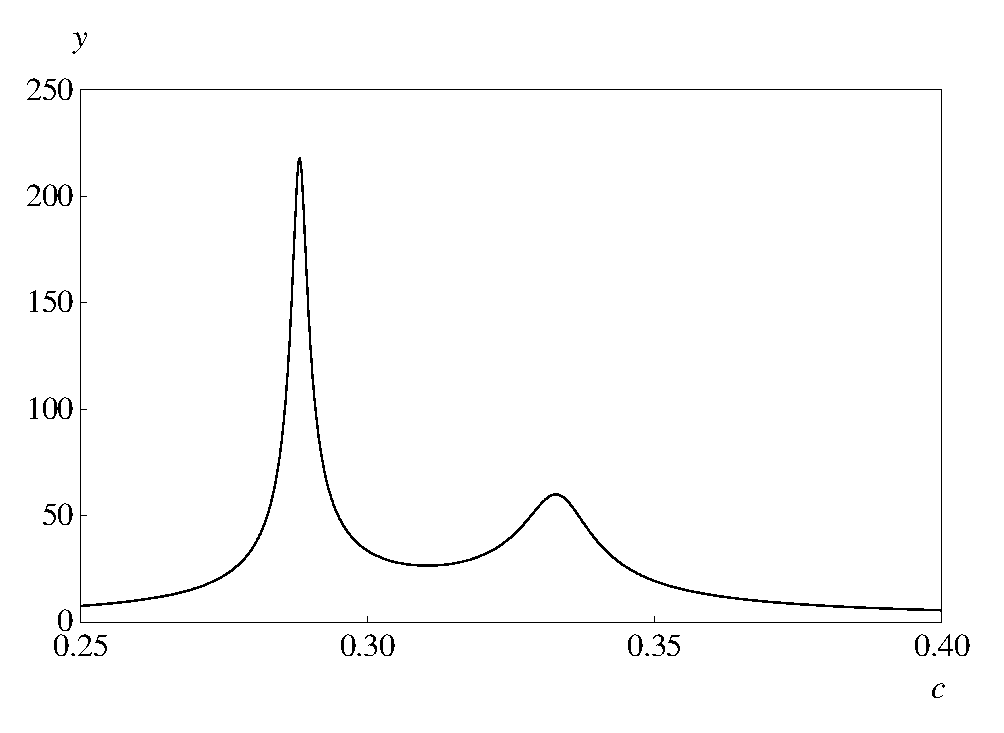
\includegraphics[width=0.95\textwidth]{images/Permit1.eps}
      \end{figure}
        \vspace{-10pt}\hfill
      \begin{minipage}[t]{0.9\textwidth}
        Залежність відносної дійсної частини ефективної проникності ($y = \varepsilon_{\rm eff}/\varepsilon_1$) від концентрації ядер $c$. 
        
        \vspace{5pt}
        Експериментальне підтверждення для ЖК систем: [S. Tomylko et al., Phys. Rev. E {\bf 92(1)} (2015) 012502]
      \end{minipage}
\end{columns}
\end{frame}

%%%%%%%%%%%%%%%%%%%%%%%%%%%%%%%%%%%%%%%%%%%%%%%%%%%%%
\begin{frame}{Ефективні критичні індекси перколяції}
\footnotesize

\vspace{-15pt}
\begin{columns}[T,onlytextwidth]
    \column{0.5\textwidth}
      \begin{figure}
        \centering
        $$x \sim (c-c_c)^t, \quad (c \to c_c+0)$$
        $$t_{\rm eff} = ln \frac{\sigma(c_2)}{\sigma(c_1)} / ln \frac{c_2-c_c}{c_1 - c_c}, \quad (c>c_c)$$
        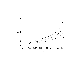
\includegraphics[width=0.99\textwidth]{images/teff.eps}
      \end{figure}
        Залежність ефективного індексу $t_{\rm eff}$ від $c_2$ при фіксованих $c_1$, $\delta=0.1$ ($c_c \approx 0.251$) та $x_2 = 5\times 10^{-5}$. Звурху вниз: $c_1 = 0.26, 0.27, 0.28$.\\
        Теорія перколяцій: $t \approx 1.3 \div 2.14$\\
        Експеримент: $t\approx 1.5 \div 2.0$ та вище

    \column{0.5\textwidth}
      \begin{figure}
        \centering
        $$x \sim (c_c-c)^{-s}, \quad (c \to c_c-0)$$
        $$s_{\rm eff} = - ln \frac{\sigma(c_2)}{\sigma(c_1)} / ln \frac{c_c-c_2}{c_c - c_1}, \quad (c<c_c)$$
        \includegraphics[width=0.99\textwidth]{images/seff.eps}
      \end{figure}
      \hfill
      \begin{minipage}[t]{0.9\textwidth}
        Залежність ефективного індексу $s_{\rm eff}$ від $x_0 = \sigma_0/\sigma_1$ при  $\delta=0.1$ ($c_c \approx 0.251$), $x_2 = 5\times 10^{-5}$, $c_1 = 0.24$ та $c_2 = 0.25$.\\
        Теорія перколяцій: $s \approx 0.75$\\
        Експеримент: $s\approx 0.7 \div 1.0$
      \end{minipage}
\end{columns}

\end{frame}


%%%%%%%%%%%%%%%%%%%%%%%%%%%%%%%%%%%%%%%%%%%%%%%%%%%%%
\subsection{Порівняння з експериментальними даними}
%{\setbeamertemplate{frame footer}{Експеримент: [I.-G. Chen, W. Johnson, J. Mat. Sci. {\bf 21} (1986) 3162]}
\begin{frame}{Порівняння з експериментальними даними з провідності}

    \scriptsize{Експеримент: [I.-G. Chen, W. Johnson, J. Mat. Sci. {\bf 21} (1986) 3162]}
    
\footnotesize
\begin{columns}[T,onlytextwidth]
    \column{0.4\textwidth}
    \vspace{10pt}
      Ефективний питомий опір зразку композита $\rm KCl-Ag$ (квадрати) та обробка згідно нашої теорії: \\
      $\sigma_0 \approx 3.15 \times 10^{-8}$~С/м; \\
      $\sigma_1 \approx 6.3 10^7$~С/м; $\sigma_2 \approx 0.3 \times 10^3$~С/м; \\
      $\delta = 0.1682$ ($c_c = 0.214$).

      \vspace{5pt}
      Середній радіус частинок $\rm Ag$: $R\approx 10$~нм. 
      
      Вимірювана товщина оболонки: $\delta \approx 0.1$.

    \column{0.6\textwidth}
      \begin{figure}
        \centering
        \includegraphics[width=0.99\textwidth]{images/grannan-sigma-fin.eps}
      \end{figure}
\end{columns}

\end{frame}
%}
%{\setbeamertemplate{frame footer}{Експеримент: [D. Grannan, J. Garland, D. Tanner, Phys. Rev. Lett. {\bf 46} (1981) 375]}

%%%%%%%%%%%%%%%%%%%%%%%%%%%%%%%%%%%%%%%%%%%%%%%%%%%%%
\begin{frame}{Порівняння з експериментальними даними з проникності}

    \scriptsize{Експеримент: [D. Grannan, J. Garland, D. Tanner, Phys. Rev. Lett. {\bf 46} (1981) 375]}
    \footnotesize

\begin{columns}[T,onlytextwidth]
    \column{0.4\textwidth}
    \vspace{10pt}
      Еффективна проникність для двох зразків $\rm KCl-Ag$ (круги й трикутники) до порога перколяції та обробка згідно нашої теорії. 
      
      \vspace{5pt}
      -- Чорні лінії:\\
      $\varepsilon_0 = 5.0$, \\
      $\delta = 0.194$, \\
      $s = 0.72$. \\
      -- Сині лінії:\\
      $\varepsilon_0 = 7.0$, \\
      $\delta = 0.150$, \\
      $s = 0.74$.
      

    \column{0.6\textwidth}
      \begin{figure}
        \centering
        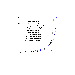
\includegraphics[width=0.99\textwidth]{images/chen-fin.eps}
      \end{figure}
\end{columns}

\end{frame}
%}

%%%%%%%%%%%%%%%%%%%%%%%%%%%%%%%%%%%%%%%%%%%%%%%%%%%%%%%%%%%%%%%%%%%%%%%%%%%%%%%%%%%%%%%%%%%
\section{Застосування підходу до аналізу диференціального метода}%%%%%%%%%%%%%%%%%%%%%%%%%%%%%%%
%%%%%%%%%%%%%%%%%%%%%%%%%%%%%%%%%%%%%%%%%%%%%%%%%%%%%%%%%%%%%%%%%%%%%%%%%%%%%%%%%%%%%%%%%%

\begin{frame}{Диференціальний метод (асиметричний підхід Бругемана)}
\footnotesize

Розглянемо систему твердих діелектричних куль в діелектричній матриці при деякій концентрації $c$ та ефективній проникності $\varepsilon$.

Моделювання в рамках {\bf асиметричного підходу Бругемана (ABM)}:

\begin{wrapfigure}{r}{0.55\textwidth}
\vspace{-20pt}
  \begin{center}
    \begin{overpic}[width=0.55\textwidth]{images/hanai-fig1.eps}
         %\put(60,70){$\rm KCl/Ag$}
    \end{overpic}
  \end{center}
\vspace{-25pt}
\end{wrapfigure}
\textbf{Електродинамічна взаємодія між новими порціями частинок, що додаються, та старими виконується за рахунок поточного ефективного середовища.}

%Зазвичай застосовується для опису діелектричних властивостей емульсій, грунту, тощо.

При зміні концентрації частинок:
\begin{equation}
     \frac{\Delta \varepsilon}{3\varepsilon} = \frac{\Delta c}{1-c} \frac{\varepsilon_1 - \varepsilon}{2\varepsilon + \varepsilon_1}  
    \quad \Rightarrow \quad
      1 - c = \frac{\varepsilon - \varepsilon_1}{\varepsilon_0 - \varepsilon_1} \left( \frac{{ \varepsilon_0}}{\varepsilon} \right)^{1/3}.
\end{equation}

При зміні концентрації матриці:
\begin{equation}
    \frac{\Delta \varepsilon}{3\varepsilon} = -\frac{\Delta c}{c} \frac{\varepsilon_0 - \varepsilon}{2\varepsilon + \varepsilon_0}  
    \quad \Rightarrow \quad
    c = \frac{\varepsilon - \varepsilon_0}{\varepsilon_1 + \varepsilon_0} \left( \frac{\varepsilon_1}{\varepsilon} \right)^{1/3}.
\end{equation}


\end{frame}
%%%%%%%%%%%%%%%%%%%%%%%%%%%%%%%%%%%%%%%%%%%%%%%%%%%%%
\begin{frame}{Побудова диференціальної схеми в рамках МКГ}
\footnotesize


\textbf{Припущення}: додавання інфінітизимальних порцій включень призводять до інфінітиземальних змін $c$ та $\varepsilon$.
\begin{equation}\label{eq:delta-Brug-diff0}
\begin{split}
  \widetilde{\delta\varepsilon}_{\rm CGA} ({\bf r}) =& (\varepsilon_0 - (\varepsilon + \Delta\varepsilon)) [1 - ({\Pi}_1 ({\bf r}) + \Delta{\Pi}_1 ({\bf r}))]\\
  &+ (\varepsilon_1 - (\varepsilon +   \Delta\varepsilon)) [{\Pi}_1 ({\bf r}) + \Delta{\Pi}_1 ({\bf r})] \\
  =& \delta\varepsilon_{\rm ABM}^{(l)} ({\bf r}) + \delta\varepsilon_{\rm ABM}^{(h)} ({\bf r}) + \delta\varepsilon_{\rm CGA} ({\bf r}),
\end{split}
\end{equation}
де, нехтуючи другими порядками малості,
%\begin{center}
\begin{tabular}{ ll } 
 $\delta\varepsilon_{\rm ABM}^{(l)} \approx -\Delta\varepsilon [1 - \Pi_1] + (\varepsilon_1 - \varepsilon) \Delta\Pi_1$ & відповідає змінам кількості частинок;\\ 
 $\delta\varepsilon_{\rm ABM}^{(h)} \approx -\Delta\varepsilon \Pi_1 - (\varepsilon_0 - \varepsilon)\Delta\Pi_1$ & відповідає змінам кількості матриці; \\ 
 $\delta\varepsilon_{\rm CGA} = (\varepsilon_0 - \varepsilon)[1 - \Pi_1] + (\varepsilon_1 - \varepsilon)\Pi_1$ & відповідає частинкам доданим раніше.
\end{tabular}
%\end{center}

Таким чином, \textbf{ефективне значення проникності при додаванні порції частинок формується за рахунок не тільки змін кількості частинок й матриці, а ще й за рахунок частинок, що додавалися раніше}.

Для отримання класичного закону ABM треба \textbf{знехтувати} внесками $\delta\varepsilon_{\rm ABM}^{(h)}$ (або $\delta\varepsilon_{\rm ABM}^{(l)}$) та $\delta\varepsilon_{\rm CGA}$:\\
--- $\delta\varepsilon_{\rm ABM}^{(h)}$ (або $\delta\varepsilon_{\rm ABM}^{(l)}$) можна знехтувати розглядаючи низько- (високо-) концентраційне наближення.\\
--- {$\delta\varepsilon_{\rm CGA}$ можна знехтувати якщо: 1) $\varepsilon_0 \approx \varepsilon$ та $\varepsilon_1 \approx \varepsilon$; 2) концентрації, що додаються досить малі; 3) $|\varepsilon_1-\varepsilon_0|$ також мале.}
\end{frame}

%%%%%%%%%%%%%%%%%%%%%%%%%%%%%%%%%%%%%%%%%%%%%%%%%%%%%
\begin{frame}{Порівняння результатів з границями Хашина-Штрікмана}

\begin{figure}[tb]
    \centering
    \includegraphics[width=0.55\textwidth]{images/hanai-fig2.eps}
    \caption{\label{fig:HSbounds}
    Концентраційна залежність $\varepsilon$ згідно з: отриманими низько- та високо-концентраційними залежностями в рамках МКГ (товсті чорні лінії 1, 2, відповідно); нижня та верхня границі Хашина-Штрікмана (тонкі лінії 3 та 4); підхід МКГ (штрихована лінія); оригінальні низько- та високо-концентраційні асиметричні підходи Бругемана (точкові лінії 5 та 6). При побудові був використаний тільки один параметр $\varepsilon_1/\varepsilon_0 = 10^2$.}
\end{figure}

\end{frame}


%%%%%%%%%%%%%%%%%%%%%%%%%%%%%%%%%%%%%%%%%%%
\section{Висновки}%%%%%%%%%%%%%%%%%%%%%%%%%
%%%%%%%%%%%%%%%%%%%%%%%%%%%%%%%%%%%%%%%%%%%

\begin{frame}{Висновки}
\footnotesize

--- Запропонована в роботі статистична модель електричного відгуку систем частинок з морфолгією тверде ядро--проникна оболонка, що базується на методі компактних груп, строга у статичному наближенні, що протестовано на екстенсивних даних числових симуляцій. 

--- Модель здатна кількісно відтворювати експериментальні дані з квазістатичної провідності твердих композитних та полімерних композитних електролітів. Одночастинкові профілі провідності ефективно враховують різні фізико-хімічні механізми зміни провідності.

--- Модель здатна кількісно описувати ефективні провідність та діелектричну проникність твердих невпорядкованих композитів в околі порогу електричної перколяції. 

--- Положення порогу електричної перколяції в рамках моделі залежить лише від геометричних параметрів оболонки.

--- Ефективні критичні індекси композитів залежать від геометричних та електричних параметрів компонентів та способу обробки експериментальних даних.

--- Диференціальна схема аналізу ефективних квазістатичних електричних параметрів диспесних систем внутрішньо непослідовна та загально обмежена.

\end{frame}


%%%%%%%%%%%%%%%%%%%%%%%%%%%%%%%%%%%%%%%%%%%%%%%%%%%%%
{\setbeamercolor{palette primary}{fg=black, bg=white}
\begin{frame}[standout]
  Дякую за увагу!
\end{frame}
}

\appendix

%%%%%%%%%%%%%%%%%%%%%%%%%%%%%%%%%%%%%%%%%%%%%%%%%%%%%
\subsection{Класичні методи дослідження та їх модифікації; сучасні методи}

%%%%%%%%%%%%%%%%%%%%%%%%%%%%%%%%%%%%%%%%%%%%%%%%%%%%%
\begin{frame}{Класичні методи дослідження: підхід Максвела-Гарнета}
\footnotesize
    Перший результат теорії гомогенізації, що дозволив обробляти експериментальні дані.
    Кожна частинка розглядається окремо в середовищі дисперсійної фази (матриці) в рамках підходу Клаузіуса-Моссотті:
    \begin{equation}\label{eq:MG}
    \frac{a_{\rm eff} - a_0}{2a_0 + a_{\rm eff}} = c \frac{a_1 - a_0}{2a_0 + a_1},
    \end{equation}
    де $c$ -- об'ємна концентрація дисперсної фази з провідністю/проникністю $a_1$, що знаходиться в матриці з проникністю $a_0$; $a_{\rm eff}$ -- ефективна провідністю/проникністю системи.\par
    [J.C. Maxwell, A Treatise on Electricity and Magnetism, Clarendon Press (1873); J.C. Maxwell-Garnett, Trans. R. Soc. Lond. {\bf 203} (1904) 385]
    \vspace{-5pt}
    \begin{columns}[T,onlytextwidth]
        \column{0.5\textwidth}
          \begin{center}
          {\it Переваги}
          \end{center}
          \vspace{-10pt}
          \begin{itemize}
              \item дуже проста модель, що дає змогу швидко оцінити ефективні властивості системи.
          \end{itemize}
    
        \column{0.5\textwidth}
          \begin{center}
          {\it Недоліки}
          \end{center}
          \vspace{-10pt}
          \begin{itemize}
              \item одночастинковий підхід; застосований при низьких концентраціях.
              \item не передбачає ефекту перколяції.
              \item для несферичних частинок на великих концентраціях дає нефізичні результати.
          \end{itemize}
    \end{columns}
\end{frame}
%%%%%%%%%%%%%%%%%%%%%%%%%%%%%%%%%%%%%%%%%%%%%%%%%%%%%
\begin{frame}{Класичні методи дослідження: теорія перколяції}

\footnotesize
    Теорія перколяції вивчає різноманітні властивості ефекту появи нескінченного кластеру зв'язаних частинок (перколяційного кластеру) в різних геомеріях: перколяція на гратках, просторова перколяція. Для статичної провідності теорія перколяції дає наступні скейлінгові співвідношення поблизу найменшої концентрації $c_c$, на якій ймовірність появи перколяційного кластеру не нульова (критична точка):
    \begin{equation}\label{eq:percolation}
        \sigma_{\rm eff} \sim \left\{ \begin{array}{ll}
            (c - c_c)^t, & c \to c_c +0\\
            (c_c - c)^{-s}, & c \to c_c -0,
        \end{array} \right.
    \end{equation}
    де $t$ та $s$ -- перколяційні критичні індекси провідності.
    
    [D. Stauffer, A. Aharony, \textit{Introduction to Percolation Theory}, Taylor \& Francis (2003)]
    \vspace{-5pt}
    \begin{columns}[T,onlytextwidth]
        \column{0.5\textwidth}
          \begin{center}
          {\it Переваги}
          \end{center}
          \vspace{-10pt}
          \begin{itemize}
              \item математично послідновний та строгий підхід до опису провідності поблизу перколяційного переходу.
          \end{itemize}
    
        \column{0.5\textwidth}
          \begin{center}
          {\it Недоліки}
          \end{center}
          \vspace{-10pt}
          \begin{itemize}
              \item зазвичай використовані моделі фізично не обґрунотвані.
              \item неуніверсальність критичних індексів.
              \item вивчає властивості тільки в околі критичної точки.
          \end{itemize}
    \end{columns}
  
\end{frame}
%%%%%%%%%%%%%%%%%%%%%%%%%%%%%%%%%%%%%%%%%%%%%%%%%%%%%
\begin{frame}{Класичні методи дослідження: підхід Бругемана}

\footnotesize
    Кожна компонента системи розглядається окремо як частинка в середовищі, властивості $a_{\rm eff}$ якого утворені всіма іншими компонентами системи та шукаються на експерименті:
    \begin{equation}\label{eq:EMA}
        (1-c) \frac{a_0 - a_{\rm eff}}{2a_{\rm eff} + a_0} + c \frac{a_1 - a_{\rm eff}}{2a_{\rm eff} + a_1} = 0.
    \end{equation}
    [D. Bruggeman, Ann. Phys. {\bf 416} (1935) 636]
    \vspace{-5pt}
    \begin{columns}[T,onlytextwidth]
        \column{0.5\textwidth}
          \begin{center}
          {\it Переваги}
          \end{center}
          \vspace{-10pt}
          \begin{itemize}
              \item дає гарні результати при малих та великих концентраціях.
              \item передбачає ефект перколяції.
          \end{itemize}
    
        \column{0.5\textwidth}
          \begin{center}
          {\it Недоліки}
          \end{center}
          \vspace{-10pt}
          \begin{itemize}
              \item теорія ефективного (самоузгодженого) поля.
              \item значення порогу та критичних індексів перколяції відповідають результатам теорії самоузгодженого поля.
              \item вважається, що геометрія форми частинок дисперсної фази та матриці співпадає.
          \end{itemize}
    \end{columns}
  
\end{frame}
%%%%%%%%%%%%%%%%%%%%%%%%%%%%%%%%%%%%%%%%%%%%%%%%%%%%%
\begin{frame}{Класичні методи дослідження: диференціальний підхід}

\footnotesize
    Додавання у систему з даною ефективною проникністю/провідністю $a$ інфінітизимальної порції включень з концентрацією $\Delta c/(1-c)$ у вільну від інших частинок область призводять до формування системи з новим ефективним відгуком $a+\Delta a$, що служить матрицею для наступних порцій. Частинки кожної порції розглядаються за правилом Максвела-Гарнета:
    \begin{equation}\label{eq:AEMA}
        \frac{\Delta a}{3a} = \frac{\Delta c}{1-c} \frac{a_1 - a}{2a + a_1} \quad\Rightarrow\quad
        1 - c = \frac{a_{\rm eff} - a_1}{a_0 - a_1} \left( \frac{{ a_0}}{a_{\rm eff}} \right)^{1/3}.
    \end{equation}
    [D. Bruggeman, Ann. Phys. {\bf 416} (1935) 636]
    \vspace{-5pt}
    \begin{columns}[T,onlytextwidth]
        \column{0.5\textwidth}
          \begin{center}
          {\it Переваги}
          \end{center}
          \vspace{-10pt}
          \begin{itemize}
              \item адекватно описує результати для емульсій типу вода/олія.
          \end{itemize}
    
        \column{0.5\textwidth}
          \begin{center}
          {\it Недоліки}
          \end{center}
          \vspace{-10pt}
          \begin{itemize}
              \item не передбачає перколяції.
              \item взаємодія між новими порціямичастинок та старими за рахунок ефективного середовища.
              \item вважається, що геометрія форми частинок дисперсної фази та матриці співпадає.
          \end{itemize}
    \end{columns}
  
\end{frame}

%%%%%%%%%%%%%%%%%%%%%%%%%%%%%%%%%%%%%%%%%%%%%%%%%%%%%
\begin{frame}{Модифікації класичних методів: Накамура, Нан, Вєчорик}
\footnotesize
    Комбінація класичних підходів Максвелла-Гарнетта і Бруггемана, застосованих до систем частинок типу ядро-оболонка.  
    
    Основні кроки: 1) Провідність кожної такої неоднорідної частинки замінюється деякою ефективною провідністю $\sigma^{*}_1$, обчислюваною для усамітненої частинки в однорідному полі.  2) Ефективна провідність системи таких частинок обчислюється в рамках класичних двофазних моделей окремо для низьких та високих концентрацій. 3) Ефективна провідність композиту $\sigma_{\rm eff}$ знаходиться зшиванням знайдених  граничних розв'язків в точці,  що відповідає максимуму $\sigma_{\rm eff}$. Це веде до появи нефізичного зламу в точці зшивання.  
    
    %гострого піку у точці максимуму\par
    % Високопровідні області моделюються оболонками навколо частинок; кожна частинка зі своєю оболонкою розглядається окремо як ``складна частинка'', ефективна провідність якої до та після максимуму $\sigma_{\rm eff}$ вважається різною задля врахування ефекту перекриття оболонок. Ефективні властивості таких частинок й матриці та $\sigma_{\rm eff}$ розраховуються комбінуючи методи Бругемана та Максвела Гарнета, ``сшиваючи'' рішення у точці максимуму.  
    [M.~Nakamura, Phys. Rev. B {\bf 29} (1984) 3691; C.-W.~Nan, Prog. Mater. Sci. \textbf{37} (1993) 1; W.~Wieczorek et al., J. Phys. Chem. {\bf 98} (1994) 6840]
  
\end{frame}
%%%%%%%%%%%%%%%%%%%%%%%%%%%%%%%%%%%%%%%%%%%%%%%%%%%%%
\begin{frame}{Модифікації класичних методів: Маклачлан}

\footnotesize
    Емпірична модель, побудована на базі класичного підходу Бругемана так, щоб поблизу порогу перколяції задовільняти перколяційним скейлінговим співвідношенням:
    \begin{equation}\label{eq:GEMA}
    (1-c) \frac{a_0^{1/s} - a_{\rm eff}^{1/s}}{Aa_{\rm
    		eff}^{1/s} + a_0^{1/s}} + c \frac{a_1^{1/t} -
    	a_{\rm eff}^{1/t}}{Aa_{\rm eff}^{1/t} + a_1^{1/t}}= 0.
    \end{equation}
    [D. McLachlan, J. Phys. C: Solid State Phys. {\bf 20} (1987) 865]
    \vspace{-5pt}
    \begin{columns}[T,onlytextwidth]
        \column{0.5\textwidth}
          \begin{center}
          {\it Переваги}
          \end{center}
          \vspace{-10pt}
          \begin{itemize}
              \item здатен відновлювати експериментальні дані для широкого класу систем типу діелектрик-провідник.
          \end{itemize}
    
        \column{0.5\textwidth}
          \begin{center}
          {\it Недоліки}
          \end{center}
          \vspace{-10pt}
          \begin{itemize}
              \item емпірична модель; не має чіткої теоретичної бази.
              \item не дає змогу аналізувати мікроструктуру системи.
          \end{itemize}
    \end{columns}

\end{frame}
%%%%%%%%%%%%%%%%%%%%%%%%%%%%%%%%%%%%%%%%%%%%%%%%%%%%%
\begin{frame}{Сучасні методи: Strong-property-fluctuation theory}

\footnotesize
    Неоднорідності в дисперсній системі розглядаються як стахостичне поле флуктуацій великої амплітуди з тим самим розподілом. Для знаходження ефективного відгуку розв'язується рівняння розповсюдження хвилі в дисперсній системі ітераційним методом. Багаточастинкові вклади розраховуються напряму; зазвичай обмежуються білокальним наближенням.
    [Ю.А. Рыжев, В.В. Тамойкин, В.И. Татарский, ЖЭТФ \textbf{48} (1965) 656; T.G. Mackay, A. Lakhtakia, W.S. Weiglhofer, Phys. Rev. E {\bf 63} (2000) 6052]
    \vspace{-5pt}
    \begin{columns}[T,onlytextwidth]
        \column{0.5\textwidth}
          \begin{center}
          {\it Переваги}
          \end{center}
          \vspace{-10pt}
          \begin{itemize}
              \item формально строгий послідовний підхід.
          \end{itemize}
    
        \column{0.5\textwidth}
          \begin{center}
          {\it Недоліки}
          \end{center}
          \vspace{-10pt}
          \begin{itemize}
              \item необхідно напряму розраховувати багаточастинкові вклади напряму; обмежуються, як правило, білокальним наближенням.
              \item для покращення здіжності ітераційної процедури постулюються певні обмеження на стахостичні поля.
          \end{itemize}
    \end{columns}

\end{frame}
%%%%%%%%%%%%%%%%%%%%%%%%%%%%%%%%%%%%%%%%%%%%%%%%%%%%%
\begin{frame}{Сучасні методи: метод компактних груп неоднорідностей}

\footnotesize
    Розв'язується рівняння розповсюдження хвилі в дисперсній системі ітераційним методом у довгохвильовому наближенні (такому, що вкладами діелектричних втрат можна знехтувати).
    Система розглядається як сукупність макроскопічних областей (компактних груп), лінійні розміри яких набагато менші ніж довжина хвилі в середовищі; ефективні властивості системи формуються властивостями компактних груп.
    Отсанні знаходяться в допоміжній матриці, вибір властивостей якої суть електродинамічна гомогенізація.
    [М.Я. Сушко, ЖЭТФ {\bf 132} (2007) 478; J. Phys. D: Appl. Phys. {\bf 42} (2009) 155410; Phys. Rev. E {\bf 96} (2017) 062121]
    \vspace{-5pt}
    \begin{columns}[T,onlytextwidth]
        \column{0.5\textwidth}
          \begin{center}
          {\it Переваги}
          \end{center}
          \vspace{-10pt}
          \begin{itemize}
              \item дозволяє уникнути деталізації багаточастинкових поляризаційних та кореляційних ефектів.
              \item дає точні результати у довгохвильовому наближенні.
              \item дуже гнучкий в плані моделювання мікроструктури.
          \end{itemize}
    
        \column{0.5\textwidth}
          \begin{center}
          {\it Недоліки}
          \end{center}
          \vspace{-10pt}
          \begin{itemize}
              \item може бути застосований лише до макроскопічно однорідних та ізотропних немагнітних дисперсних систем.
              \item теорія є аналогом підходу самоузгодженого поля.
              \item теорія розвинена лише для діелектричних систем.
          \end{itemize}
    \end{columns}

\end{frame}
%%%%%%%%%%%%%%%%%%%%%%%%%%%%%%%%%%%%
\begin{frame}{Границі Хашина-Штрікмана}

\footnotesize
    Один з точних та перших результатів теорії гомогенізації, що основується на варіаціному принципі, й дає верхню $a^{+}$ та нижню $a^{-}$ границі значень провідності ($a=\sigma$) та проникності ($a=\varepsilon$) двофазних дисперсних систем на всьому концентраційному проміжку:
    \begin{equation}\label{eq:HS-bounds}
    \begin{split}
    	&a^{-} = a_1 + \frac{3c_2 a_1(a_2-a_1)}{3a_1 + c_2(a_2-a_1)};\\
    	&a^{+} = a_2 + \frac{3c_1 a_2(a_1-a_2)}{3a_2 + c_1(a_1-a_2)},
    \end{split}
    \end{equation}
    де $c_{1}$, $c_2=(1-c_1)$ та $a_{1}$,$a_{2}$ -- об'ємні концентрації та провідності/проникності першої та другої компонент, відповідно.\par
    [Z. Hashin and S. Shtrikman, J. Appl. Phys. {\bf 33} (1962) 3125]
    \vspace{-5pt}
    \begin{columns}[T,onlytextwidth]
        \column{0.5\textwidth}
          \begin{center}
          {\it Переваги}
          \end{center}
          \vspace{-10pt}
          \begin{itemize}
              \item дозволяє тестувати нові теорії на сумісність.
          \end{itemize}
    
        \column{0.5\textwidth}
          \begin{center}
          {\it Недоліки}
          \end{center}
          \vspace{-10pt}
          \begin{itemize}
              \item обробка експериментальних даних неможлива для майже всіх систем.
          \end{itemize}
    \end{columns}
  
\end{frame}

\end{document}
